%%%% Paramétrage du TD %%%%
\def\xxactivite{\ifcolle Colle \else Application 02 \fi \ifprof -- Corrigé \else \fi }
\def\xxauteur{\textsl{Xavier Pessoles}}


\def\xxnumchapitre{Révisions 4 \vspace{.2cm}}
\def\xxchapitre{\hspace{.12cm} Modélisation des systèmes du premier et du deuxième ordre}

\def\xxcompetences{%
\vspace{-.5cm}
\footnotesize{
\textsl{%
\textbf{Savoirs et compétences :}\\
\vspace{-.2cm}
\begin{itemize}[label=\ding{112},font=\color{ocre}] 
\item ...
\end{itemize}}}}

\def\xxfigures{
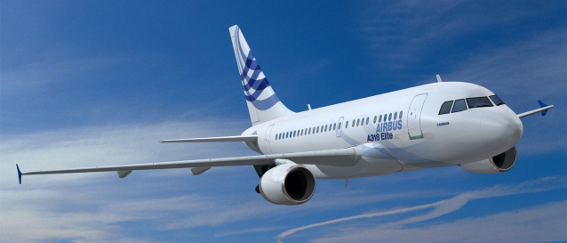
\includegraphics[width=.8\linewidth]{image1.png}%images/prot_01}
}%figues de la page de garde

\def\xxonglet{\textsf{Cy 01 -- Rév 4}}

\def\xxtitreexo{Freinage d'Airbus }
\def\xxsourceexo{David Violeau}

\iflivret
\pagestyle{empty}


%%%%%%%% PAGE DE GARDE COURS
\ifcours
% ==== BANDEAU DES TITRES ==== 
\begin{tikzpicture}[remember picture,overlay]
\node at (current page.north west)
{\begin{tikzpicture}[remember picture,overlay]
\node[anchor=north west,inner sep=0pt] at (0,0) {\includegraphics[width=\paperwidth]{\thechapterimage}};
\draw[anchor=west] (-2cm,-8cm) node [line width=2pt,rounded corners=15pt,draw=ocre,fill=white,fill opacity=0.6,inner sep=40pt]{\strut\makebox[22cm]{}};
\draw[anchor=west] (1cm,-8cm) node {\huge\sffamily\bfseries\color{black} %
\begin{minipage}{1cm}
\rotatebox{90}{\LARGE\sffamily\textsc{\color{ocre}\textbf{\xxnumpartie}}}
\end{minipage} \hfill
\begin{minipage}[c]{14cm}
\begin{titrepartie}
\begin{flushright}
\renewcommand{\baselinestretch}{1.1} 
\Large\sffamily\textsc{\textbf{\xxpartie}}
\renewcommand{\baselinestretch}{1} 
\end{flushright}
\end{titrepartie}
\end{minipage} \hfill
\begin{minipage}[c]{3.5cm}
{\large\sffamily\textsc{\textbf{\color{ocre} \discipline}}}
\end{minipage} 
 };
\end{tikzpicture}};
\end{tikzpicture}
% ==== FIN BANDEAU DES TITRES ==== 


% ==== ONGLET 
\begin{tikzpicture}[overlay]
\node[shape=rectangle, 
      rounded corners = .25 cm,
	  draw= ocre,
	  line width=2pt, 
	  fill = ocre!10,
	  minimum width  = 2.5cm,
	  minimum height = 3cm,] at (18.3cm,0) {};
\node at (17.7cm,0) {\rotatebox{90}{\textbf{\Large\color{ocre}{\classe}}}};
%{};
\end{tikzpicture}
% ==== FIN ONGLET 


\vspace{3.5cm}

\begin{tikzpicture}[remember picture,overlay]
\draw[anchor=west] (-2cm,-6cm) node {\huge\sffamily\bfseries\color{black} %
\begin{minipage}{2cm}
\begin{center}
\LARGE\sffamily\textsc{\color{ocre}\textbf{\xxactivite}}
\end{center}
\end{minipage} \hfill
\begin{minipage}[c]{15cm}
\begin{titrechapitre}
\renewcommand{\baselinestretch}{1.1} 
\Large\sffamily\textsc{\textbf{\xxnumchapitre}}

\Large\sffamily\textsc{\textbf{\xxchapitre}}
\vspace{.5cm}

\renewcommand{\baselinestretch}{1} 
\normalsize\normalfont
\xxcompetences
\end{titrechapitre}
\end{minipage}  };
\end{tikzpicture}
\vfill

\begin{flushright}
\begin{minipage}[c]{.3\linewidth}
\begin{center}
\xxfigures
\end{center}
\end{minipage}\hfill
\begin{minipage}[c]{.6\linewidth}
\startcontents
%\printcontents{}{1}{}
\printcontents{}{1}{}
\end{minipage}
\end{flushright}

\begin{tikzpicture}[remember picture,overlay]
\draw[anchor=west] (4.5cm,-.7cm) node {
\begin{minipage}[c]{.2\linewidth}
\begin{flushright}

\includegraphics[width=2cm]{logoCC}
\end{flushright}
\end{minipage}
\begin{minipage}[c]{.2\linewidth}
\textsl{\xxauteur} \\
\textsl{\classe}
\end{minipage}
 };
\end{tikzpicture}

\newpage
\pagestyle{fancy}

%\newpage
%\pagestyle{fancy}

\else
\fi
%% FIN PAGE DE GARDE DES COURS

%%%%%%%% PAGE DE GARDE TD
\iftd

% BANDEAU EXO
\iflivret % SI LIVRET
\begin{tikzpicture}[remember picture,overlay]
\draw[anchor=west] (-2cm,-3.3cm) node {\huge\sffamily\bfseries\color{black} %
\begin{minipage}{5cm}
\begin{center}
\LARGE\sffamily\color{ocre}\textbf{\textsc{\xxactivite}}

\begin{center}
\xxfigures
\end{center}

\end{center}
\end{minipage} \hfill
\begin{minipage}[c]{12cm}
\begin{titrechapitre}
\renewcommand{\baselinestretch}{1.1} 
\large\sffamily\textbf{\textsc{\xxtitreexo}}

\small\sffamily{\textbf{\textit{\color{black!70}\xxsourceexo}}}
\vspace{.5cm}

\renewcommand{\baselinestretch}{1} 
\normalsize\normalfont
\xxcompetences
\end{titrechapitre}
\end{minipage}};
\end{tikzpicture}
\else % ELSE NOT LIVRET
\begin{tikzpicture}[remember picture,overlay]
\draw[anchor=west] (-2cm,-4.5cm) node {\huge\sffamily\bfseries\color{black} %
\begin{minipage}{5cm}
\begin{center}
\LARGE\sffamily\color{ocre}\textbf{\textsc{\xxactivite}}

\begin{center}
\xxfigures
\end{center}

\end{center}
\end{minipage} \hfill
\begin{minipage}[c]{12cm}
\begin{titrechapitre}
\renewcommand{\baselinestretch}{1.1} 
\large\sffamily\textbf{\textsc{\xxtitreexo}}

\small\sffamily{\textbf{\textit{\color{black!70}\xxsourceexo}}}
\vspace{.5cm}

\renewcommand{\baselinestretch}{1} 
\normalsize\normalfont
\xxcompetences
\end{titrechapitre}
\end{minipage}};
\end{tikzpicture}

\fi

\else   % FIN IF TD
\fi


%%%%%%%% PAGE DE GARDE FICHE
\iffiche
\begin{tikzpicture}[remember picture,overlay]
\node at (current page.north west)
{\begin{tikzpicture}[remember picture,overlay]
\draw[anchor=west] (-2cm,-2.25cm) node [line width=2pt,rounded corners=15pt,draw=ocre,fill=white,fill opacity=0.6,inner sep=40pt]{\strut\makebox[22cm]{}};
\draw[anchor=west] (1cm,-2.25cm) node {\huge\sffamily\bfseries\color{black} %
\begin{minipage}{1cm}
\rotatebox{90}{\LARGE\sffamily\textsc{\color{ocre}\textbf{\xxnumpartie}}}
\end{minipage} \hfill
\begin{minipage}[c]{14cm}
\begin{titrepartie}
\begin{flushright}
\renewcommand{\baselinestretch}{1.1} 
\large\sffamily\textsc{\textbf{\xxpartie} \\} 

\vspace{.2cm}

\normalsize\sffamily\textsc{\textbf{\xxnumchapitre -- \xxchapitre}}
\renewcommand{\baselinestretch}{1} 
\end{flushright}
\end{titrepartie}
\end{minipage} \hfill
\begin{minipage}[c]{3.5cm}
{\large\sffamily\textsc{\textbf{\color{ocre} \discipline}}}
\end{minipage} 
 };
\end{tikzpicture}};
\end{tikzpicture}

\iflivret % SI LIVRET
\begin{tikzpicture}[overlay]
\node[shape=rectangle, 
      rounded corners = .25 cm,
	  draw= ocre,
	  line width=2pt, 
	  fill = ocre!10,
	  minimum width  = 2.5cm,
	  minimum height = 2.5cm,] at (18.5cm,.5cm) {};
\node at (17.9cm,.5cm) {\rotatebox{90}{\textsf{\textbf{\large\color{ocre}{\classe}}}}};
%{};
\end{tikzpicture}
\else  % SI PAS LIVRET
\iftd %% SI TD et PAS LIVRET
\begin{tikzpicture}[overlay]
\node[shape=rectangle, 
      rounded corners = .25 cm,
	  draw= ocre,
	  line width=2pt, 
	  fill = ocre!10,
	  minimum width  = 2.5cm,
	  minimum height = 2.5cm,] at (18.6cm,0.9cm) {};
\node at (18cm,0.9cm) {\rotatebox{90}{\textsf{\textbf{\large\color{ocre}{\classe}}}}};
%{};
\end{tikzpicture}

\else % FIN DU SI TD PAS LIVRET 
\begin{tikzpicture}[overlay]
\node[shape=rectangle, 
      rounded corners = .25 cm,
	  draw= ocre,
	  line width=2pt, 
	  fill = ocre!10,
	  minimum width  = 2.5cm,
%	  minimum height = 2.5cm,] at (18.5cm,1.1cm) {};
	  minimum height = 2.5cm,] at (18.6cm,0.5cm) {};
\node at (18cm,0.5cm) {\rotatebox{90}{\textsf{\textbf{\large\color{ocre}{\classe}}}}};
%{};
\end{tikzpicture}
\fi
\fi
\else
\fi



\else
\pagestyle{empty}


%%%%%%%% PAGE DE GARDE COURS
\ifcours
% ==== BANDEAU DES TITRES ==== 
\begin{tikzpicture}[remember picture,overlay]
\node at (current page.north west)
{\begin{tikzpicture}[remember picture,overlay]
\node[anchor=north west,inner sep=0pt] at (0,0) {\includegraphics[width=\paperwidth]{\thechapterimage}};
\draw[anchor=west] (-2cm,-8cm) node [line width=2pt,rounded corners=15pt,draw=ocre,fill=white,fill opacity=0.6,inner sep=40pt]{\strut\makebox[22cm]{}};
\draw[anchor=west] (1cm,-8cm) node {\huge\sffamily\bfseries\color{black} %
\begin{minipage}{1cm}
\rotatebox{90}{\LARGE\sffamily\textsc{\color{ocre}\textbf{\xxnumpartie}}}
\end{minipage} \hfill
\begin{minipage}[c]{14cm}
\begin{titrepartie}
\begin{flushright}
\renewcommand{\baselinestretch}{1.1} 
\Large\sffamily\textsc{\textbf{\xxpartie}}
\renewcommand{\baselinestretch}{1} 
\end{flushright}
\end{titrepartie}
\end{minipage} \hfill
\begin{minipage}[c]{3.5cm}
{\large\sffamily\textsc{\textbf{\color{ocre} \discipline}}}
\end{minipage} 
 };
\end{tikzpicture}};
\end{tikzpicture}
% ==== FIN BANDEAU DES TITRES ==== 


% ==== ONGLET 
\begin{tikzpicture}[overlay]
\node[shape=rectangle, 
      rounded corners = .25 cm,
	  draw= ocre,
	  line width=2pt, 
	  fill = ocre!10,
	  minimum width  = 2.5cm,
	  minimum height = 3cm,] at (18.3cm,0) {};
\node at (17.7cm,0) {\rotatebox{90}{\textbf{\Large\color{ocre}{\classe}}}};
%{};
\end{tikzpicture}
% ==== FIN ONGLET 


\vspace{3.5cm}

\begin{tikzpicture}[remember picture,overlay]
\draw[anchor=west] (-2cm,-6cm) node {\huge\sffamily\bfseries\color{black} %
\begin{minipage}{2cm}
\begin{center}
\LARGE\sffamily\textsc{\color{ocre}\textbf{\xxactivite}}
\end{center}
\end{minipage} \hfill
\begin{minipage}[c]{15cm}
\begin{titrechapitre}
\renewcommand{\baselinestretch}{1.1} 
\Large\sffamily\textsc{\textbf{\xxnumchapitre}}

\Large\sffamily\textsc{\textbf{\xxchapitre}}
\vspace{.5cm}

\renewcommand{\baselinestretch}{1} 
\normalsize\normalfont
\xxcompetences
\end{titrechapitre}
\end{minipage}  };
\end{tikzpicture}
\vfill

\begin{flushright}
\begin{minipage}[c]{.3\linewidth}
\begin{center}
\xxfigures
\end{center}
\end{minipage}\hfill
\begin{minipage}[c]{.6\linewidth}
\startcontents
%\printcontents{}{1}{}
\printcontents{}{1}{}
\end{minipage}
\end{flushright}

\begin{tikzpicture}[remember picture,overlay]
\draw[anchor=west] (4.5cm,-.7cm) node {
\begin{minipage}[c]{.2\linewidth}
\begin{flushright}

\includegraphics[width=2cm]{logoCC}
\end{flushright}
\end{minipage}
\begin{minipage}[c]{.2\linewidth}
\textsl{\xxauteur} \\
\textsl{\classe}
\end{minipage}
 };
\end{tikzpicture}

\newpage
\pagestyle{fancy}

%\newpage
%\pagestyle{fancy}

\else
\fi
%% FIN PAGE DE GARDE DES COURS

%%%%%%%% PAGE DE GARDE TD
\iftd

% BANDEAU EXO
\iflivret % SI LIVRET
\begin{tikzpicture}[remember picture,overlay]
\draw[anchor=west] (-2cm,-3.3cm) node {\huge\sffamily\bfseries\color{black} %
\begin{minipage}{5cm}
\begin{center}
\LARGE\sffamily\color{ocre}\textbf{\textsc{\xxactivite}}

\begin{center}
\xxfigures
\end{center}

\end{center}
\end{minipage} \hfill
\begin{minipage}[c]{12cm}
\begin{titrechapitre}
\renewcommand{\baselinestretch}{1.1} 
\large\sffamily\textbf{\textsc{\xxtitreexo}}

\small\sffamily{\textbf{\textit{\color{black!70}\xxsourceexo}}}
\vspace{.5cm}

\renewcommand{\baselinestretch}{1} 
\normalsize\normalfont
\xxcompetences
\end{titrechapitre}
\end{minipage}};
\end{tikzpicture}
\else % ELSE NOT LIVRET
\begin{tikzpicture}[remember picture,overlay]
\draw[anchor=west] (-2cm,-4.5cm) node {\huge\sffamily\bfseries\color{black} %
\begin{minipage}{5cm}
\begin{center}
\LARGE\sffamily\color{ocre}\textbf{\textsc{\xxactivite}}

\begin{center}
\xxfigures
\end{center}

\end{center}
\end{minipage} \hfill
\begin{minipage}[c]{12cm}
\begin{titrechapitre}
\renewcommand{\baselinestretch}{1.1} 
\large\sffamily\textbf{\textsc{\xxtitreexo}}

\small\sffamily{\textbf{\textit{\color{black!70}\xxsourceexo}}}
\vspace{.5cm}

\renewcommand{\baselinestretch}{1} 
\normalsize\normalfont
\xxcompetences
\end{titrechapitre}
\end{minipage}};
\end{tikzpicture}

\fi

\else   % FIN IF TD
\fi


%%%%%%%% PAGE DE GARDE FICHE
\iffiche
\begin{tikzpicture}[remember picture,overlay]
\node at (current page.north west)
{\begin{tikzpicture}[remember picture,overlay]
\draw[anchor=west] (-2cm,-2.25cm) node [line width=2pt,rounded corners=15pt,draw=ocre,fill=white,fill opacity=0.6,inner sep=40pt]{\strut\makebox[22cm]{}};
\draw[anchor=west] (1cm,-2.25cm) node {\huge\sffamily\bfseries\color{black} %
\begin{minipage}{1cm}
\rotatebox{90}{\LARGE\sffamily\textsc{\color{ocre}\textbf{\xxnumpartie}}}
\end{minipage} \hfill
\begin{minipage}[c]{14cm}
\begin{titrepartie}
\begin{flushright}
\renewcommand{\baselinestretch}{1.1} 
\large\sffamily\textsc{\textbf{\xxpartie} \\} 

\vspace{.2cm}

\normalsize\sffamily\textsc{\textbf{\xxnumchapitre -- \xxchapitre}}
\renewcommand{\baselinestretch}{1} 
\end{flushright}
\end{titrepartie}
\end{minipage} \hfill
\begin{minipage}[c]{3.5cm}
{\large\sffamily\textsc{\textbf{\color{ocre} \discipline}}}
\end{minipage} 
 };
\end{tikzpicture}};
\end{tikzpicture}

\iflivret % SI LIVRET
\begin{tikzpicture}[overlay]
\node[shape=rectangle, 
      rounded corners = .25 cm,
	  draw= ocre,
	  line width=2pt, 
	  fill = ocre!10,
	  minimum width  = 2.5cm,
	  minimum height = 2.5cm,] at (18.5cm,.5cm) {};
\node at (17.9cm,.5cm) {\rotatebox{90}{\textsf{\textbf{\large\color{ocre}{\classe}}}}};
%{};
\end{tikzpicture}
\else  % SI PAS LIVRET
\iftd %% SI TD et PAS LIVRET
\begin{tikzpicture}[overlay]
\node[shape=rectangle, 
      rounded corners = .25 cm,
	  draw= ocre,
	  line width=2pt, 
	  fill = ocre!10,
	  minimum width  = 2.5cm,
	  minimum height = 2.5cm,] at (18.6cm,0.9cm) {};
\node at (18cm,0.9cm) {\rotatebox{90}{\textsf{\textbf{\large\color{ocre}{\classe}}}}};
%{};
\end{tikzpicture}

\else % FIN DU SI TD PAS LIVRET 
\begin{tikzpicture}[overlay]
\node[shape=rectangle, 
      rounded corners = .25 cm,
	  draw= ocre,
	  line width=2pt, 
	  fill = ocre!10,
	  minimum width  = 2.5cm,
%	  minimum height = 2.5cm,] at (18.5cm,1.1cm) {};
	  minimum height = 2.5cm,] at (18.6cm,0.5cm) {};
\node at (18cm,0.5cm) {\rotatebox{90}{\textsf{\textbf{\large\color{ocre}{\classe}}}}};
%{};
\end{tikzpicture}
\fi
\fi
\else
\fi



\fi
\setlength{\columnseprule}{.1pt}

\pagestyle{fancy}
\thispagestyle{plain}


\vspace{4cm}

\def\columnseprulecolor{\color{ocre}}
\setlength{\columnseprule}{0.4pt} 

%%%%%%%%%%%%%%%%%%%%%%%
\ifprof
\else
\begin{multicols}{2}
\fi

\section*{Présentation du système}
\ifprof
\else
Le freinage est une des fonctions vitales d’un avion, au même titre que la propulsion ou la sustentation. C’est grâce à lui que l’avion peut s’immobiliser après l’atterrissage, circuler
au sol en toute sécurité mais également s’arrêter en cas d’urgence lors d’une interruption de décollage alors que l’avion est à pleine charge de carburant et lancé à la vitesse de décollage (même si le risque est de l’ordre de 1 pour 1 million de décollages). 
%Outre les freins, le pilote peut aussi actionner les inverseurs de poussée des moteurs et les aérofreins.
%On s'intéresse au système de freinage des roues de l’Airbus A318, avion commercial de 120 places et de rayon d’action de 3240 km. La vitesse de décollage est estimée à 240 km/h. Pour
%les atterrisseurs, on distingue (voir figure 2) :
%\begin{itemize}
% \item  le train avant qui, en dehors de l’appui, est orientable ce qui lui permet d’agir sur les trajectoires au sol mais qui n’est pas équipé de freins;
%\item les deux trains principaux au niveau des ailes, chacun portant deux roues freinées indépendamment. 
%\end{itemize}
%
%%\begin{minipage}[c]{.5\linewidth}
%\begin{center}
%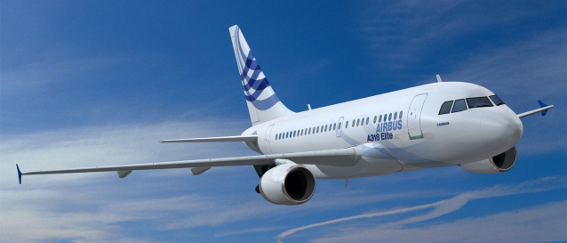
\includegraphics[width=.85\linewidth]{image1.png}
%
%\textbf{Figure 1 :} Airbus A318
%\end{center}
%%\end{minipage}\hfill
%%\begin{minipage}[c]{.47\linewidth}
%\begin{center}
%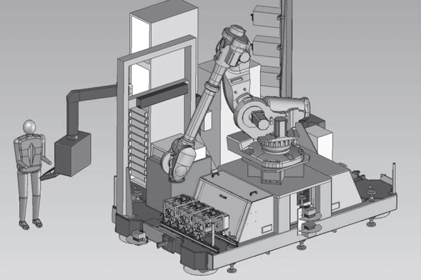
\includegraphics[width=.95\linewidth]{image2.png}
%
%\textbf{Figure 2 :} Train d'atterrissage
%\end{center}
%
%%\subsection*{Description du système de freinage}
%%
%%    Il existe deux modes de commande du système de freinage :
%%\begin{itemize}
%% \item le \textbf{mode normal} (Normal Braking) contrôlé par un ordinateur dénommé BSCU
%%(Braking/Steering Control Unit). Le BSCU contrôle les servovalves (une par roue) qui
%%alimentent les pistons presseurs. Ces pistons exercent alors une action sur les roues qui
%%diminue alors la vitesse de l'avion. La pression hydraulique est fournie par le groupe hydraulique
%%principal;
%%\item le \textbf{mode alternatif} (Alternate braking) contrôlé par un ordinateur dénommé
%%ABCU (Alternate Braking Control Unit). Ce mode prend automatiquement la relève du mode
%%normal s’il y a dysfonctionnement de ce dernier ou si le contrôle anti-dérapage (Anti-Skid) de l’avion est supprimé. En mode alternatif, la pression hydraulique est fournie par
%%un groupe hydraulique secondaire.
%%\end{itemize}
%%
%%
%%
%%%\begin{minipage}[c]{.3\linewidth}
%%\begin{center}
%%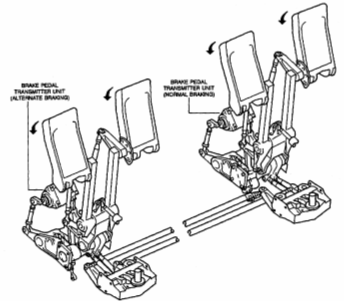
\includegraphics[width=.95\linewidth]{image3.png}
%%
%%\textbf{Figure 3 :} Pédales de frein
%%\end{center}
%%   
%%\begin{center}
%%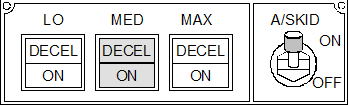
\includegraphics[width=.95\linewidth]{image4.png}
%%
%%\textbf{Figure 4}
%%\end{center}            
%%
%%%\end{minipage}\hfill
%%%\begin{minipage}[c]{.67\linewidth}
%%En mode normal, il est possible de commander le freinage de deux façons
%%différentes :
%%\begin{itemize}
%% \item soit \textbf{manuellement} par appui sur les pédales de frein (voir figure 3) : pour chaque pilote, les pédales gauche et droite sont indépendantes. L’appui sur la pédale gauche agit sur le freinage des roues du train principal gauche, l’appui sur celle de droite agit sur le freinage des roues du train principal droit. Les unités de transmission (Brake Pedal Transmitter Unit) situées sous les pédales émettent des signaux électriques vers le BSCU ou vers l’ABCU proportionnels à la course des pédales de frein;
%%\item soit \textbf{automatiquement} suivant trois modes de décélération : LO, MED, MAX. La sélection se fait à partir de trois boutons situés sur le tableau de bord (voir figure 4). Le mode manuel est rétabli si le pilote, en appuyant sur les pédales de frein, génère une consigne de
%%décélération $a_p$ supérieure à la consigne de décélération $a_c$ du mode automatique sélectionné.
%%\end{itemize}                                                    
%%%\end{minipage}
%%
%%%\vspace{.25cm} 
%%
%%Les modes LO et MED sont utilisés lors de l’atterrissage. Ils correspondent
%%respectivement à une
%%décélération de l’avion de $-1,7 ms^{-2}$ et de $-3 ms^{-2}$. Le mode MAX est
%%exclusivement sélectionné lors du
%%décollage, en cas d’interruption de ce dernier. Il correspond à une décélération
%%théorique de $-10 ms^{-2}$
%%supérieure à la décélération maximale de l’avion.
%%
%%En mode normal (manuel ou automatique), le BSCU contrôle l’anti-dérapage (Anti
%%Skid) de chaque roue
%%tant que la vitesse de l’avion est supérieure à $5\;m/s$.
%%En mode alternatif, seule la commande manuelle est disponible avec ou sans
%%anti-dérapage.
%\fi
%\section*{Description fonctionnelle du système de freinage}
%
%
%%On donne ci-dessous le SADT de niveau A-0 qui décrit la fonction principale du système de freinage.
%%
%%\begin{center}
%%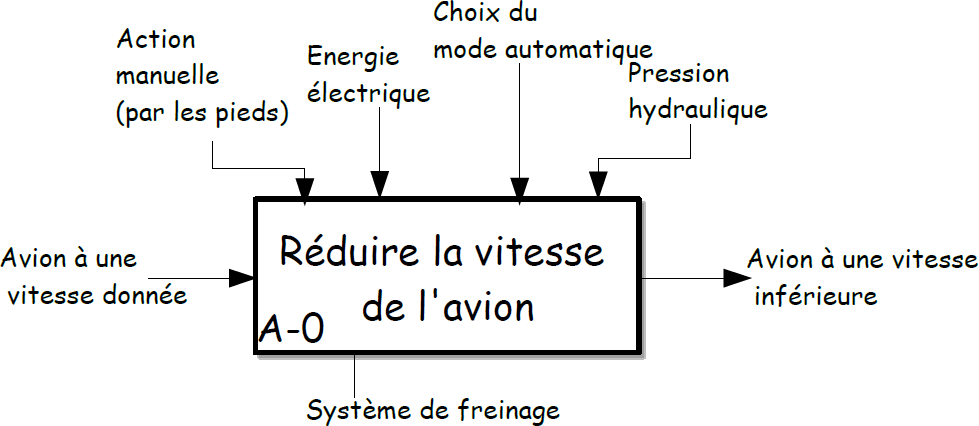
\includegraphics[width=.5\linewidth]{image5.png}
%%\end{center}
%%
%%\subparagraph{}
%%\textit{Compléter à partir des explications précédentes et du SADT A-0, le SADT de niveau A0.}
%%
%\ifprof
%\else
%On s'intéresse dans toute la suite du sujet uniquement au mode de décélération automatique du mode normal, qui consiste à asservir en décélération le freinage de l'avion.
%Bien que les variables manipulées par le BSCU soient des variables numériques, on les considèrera, par la suite, comme étant analogiques. Le système est donc, sur le plan théorique, supposé linéaire, continu et invariant.
%
%L'utilisateur donne une consigne numérique $a_c(t)$ qui est comparée à la valeur numérique $a_m(t)$ fournie par l'accéléromètre, image de la décélération réelle $a(t)$. Le BSCU génère à partir de cet écart $\varepsilon(t)$ , une commande $i(t)$ pour la servovalve. Celle-ci fournit alors la pression $p_h(t)$ aux freins qui entraîne alors la décélération $a(t)$ de l'avion.
%\fi
%
%\subparagraph{}
%\textit{Réaliser un schéma-bloc fonctionnel de l'asservissement en décélération à partir des
%indications ci-dessus. On prendra $a_c(t)$ comme entrée et $a(t)$ comme sortie.}
%
%\ifprof
%\begin{corrige}
%\begin{center}
% 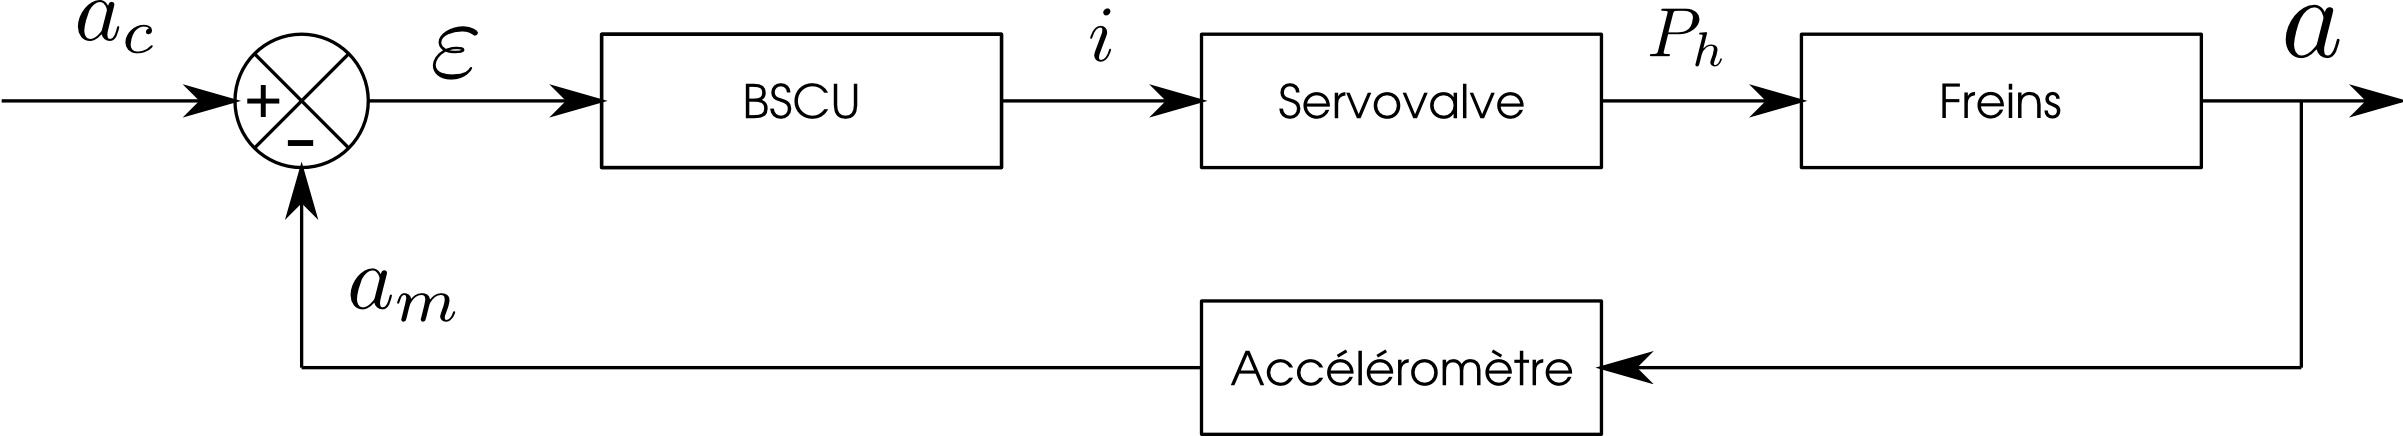
\includegraphics[width=.8\linewidth]{blocs}
%\end{center}
%\end{corrige}
%\else
%\fi
%%\begin{center}
%%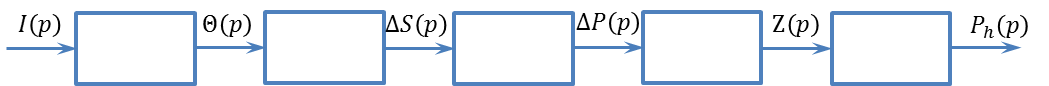
\includegraphics[width=.95\linewidth]{schema_bloc_vierge.png}
%%\end{center}
%

\fi
\section*{Modélisation du système de freinage}

On souhaite définir un modèle pour l'asservissement en décélération. Pour cela, on propose de déterminer une fonction de transfert pour tous les constituants.




\subsection*{Modélisation de la servovalve}
\ifprof
\else

Une servovalve électrohydraulique est un appareil qui convertit une grandeur électrique (courant ou tension) en une grandeur hydraulique proportionnelle (débit ou pression).
%La servovalve la plus utilisée est la servovalve en débit ou pression à 2 étages. Elle est constituée de trois éléments :
%\begin{itemize}
%\item un actionneur de type moteur électrique;
%\item un amplificateur hydraulique constitué d’un mécanisme buse-palette;
%\item un tiroir de distribution.
%\end{itemize}

\begin{center}
\begin{tabular}{cc}
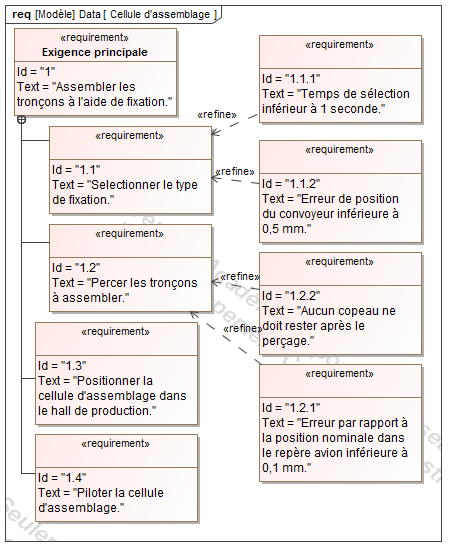
\includegraphics[width=.45\linewidth]{image6.png}&
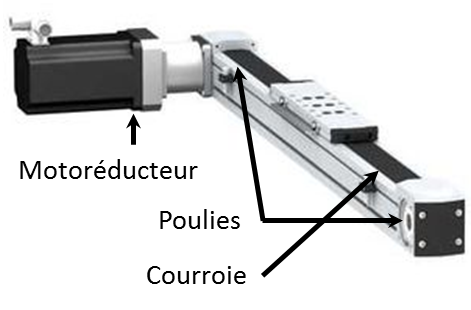
\includegraphics[width=.45\linewidth]{image7.png}
\end{tabular}
\end{center}
%
%L’armature du moteur à courant continu se prolonge dans l’entrefer d’un circuit magnétique. Le passage d’un courant continu dans les deux bobines situées de part et d’autre de l’armature provoque le basculement de cette dernière d’un angle $\theta$.
%
%L’armature est solidaire d’une palette plongeant dans l’amplificateur hydraulique et dont l’extrémité est située entre deux buses. Le mouvement de rotation de l’ensemble armature-palette vient étrangler le débit fluide traversant l’une ou l’autre des buses. La pression différentielle ainsi créée se répercute aux deux extrémités du tiroir du distributeur et provoque son déplacement.
%
%Ce tiroir possède trois orifices de contrôle, $P_a$ (Alimentation), $P_h$ (Utilisation), $R$ (Retour à la bâche). La pression $P_h$ est proportionnelle au déplacement du tiroir compté à partir de la position zéro (position du milieu).
%
%A titre indicatif, le diamètre $d$ des buses est de l’ordre de quelques dixièmes de millimètres et l’écart $e$ entre la buse et la palette de l’ordre de quelques centièmes de millimètres.

On donne ci-dessous la caractéristique reliant l'intensité $i(t)$ du moteur à l'angle $\theta(t)$ dont bascule l'armature.

\begin{center}
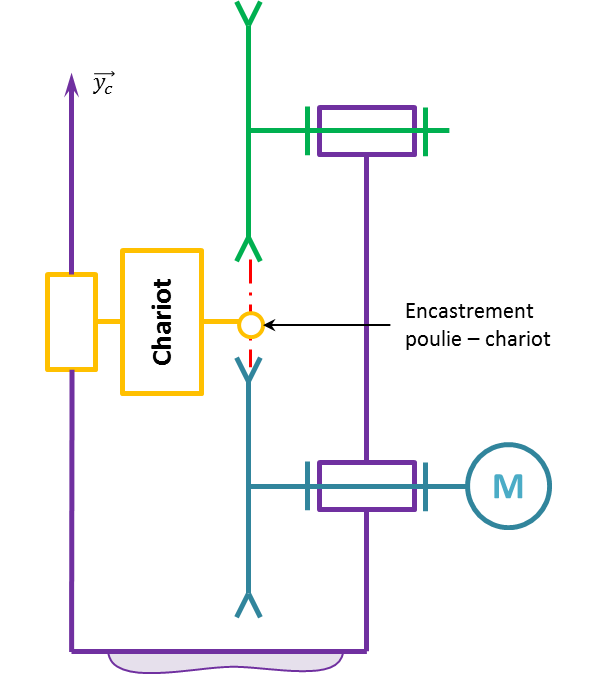
\includegraphics[width=.8\linewidth]{image8.png}
\end{center}

\fi



\subparagraph{}
\textit{Que peut-on dire de cette caractéristique sur tout le domaine de variation de $i(t)$ ? Sachant que $\theta$ est très petit (varie autour de 0), on utilise la relation suivante $\theta(t)=K_1i(t)$.  Déterminer la valeur de $K_1$ à partir de la courbe.}

\ifprof
\begin{corrige}
Cette courbe est non linéaire sur tout le domaine de variation de $i$. Comme
$\theta$ est très petit, on peut linéariser la courbe au voisinage de 0. La
valeur $K_1$ correspond donc à la pente  de la courbe. En conséquence,
$K_1=1\;rad\cdot A^{-1}$. 
\end{corrige}
\else 


On admet que, pour le système buse-palette, la rotation d'angle $\theta$ de la palette se traduit par un
accroissement ou diminution de la distance buse-palette. Les sections de fuite sont alors augmentées ou
diminuées, ce qui entraîne une augmentation ou diminution des pressions $P_A$ et $P_B$ proportionnelle à
$\Delta S$.

\begin{center}
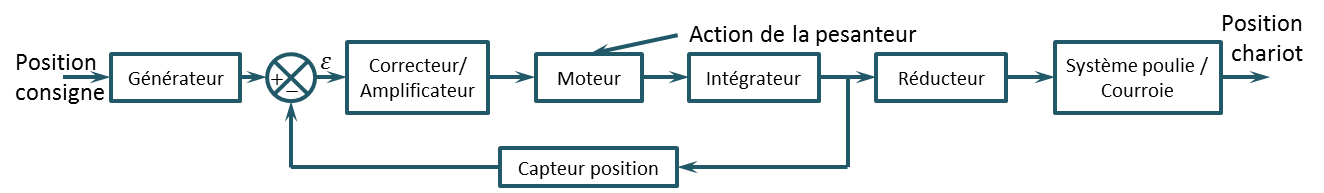
\includegraphics[width=.8\linewidth]{image9.png}
\end{center}

On peut alors définir les relations suivantes :
$$\Delta S (t)=K_2 \theta (t) $$
$$\Delta P (t)=K_3 \Delta  S(t)$$

Cette pression différentielle permet de mettre en mouvement le tiroir de la servovalve.

En situation repos, lorsque $P_A=P_B=P_0$, le tiroir est en position milieu, $z = 0$ ( cf figure ci-dessous).

\begin{center}
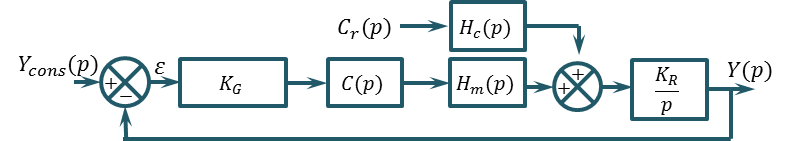
\includegraphics[width=.5\linewidth]{image10.png}

\textit{Tiroir en position repos}
\end{center}


En position travail, la pression différentielle se répercute aux extrémités du tiroir et provoque son
déplacement.

\begin{center}
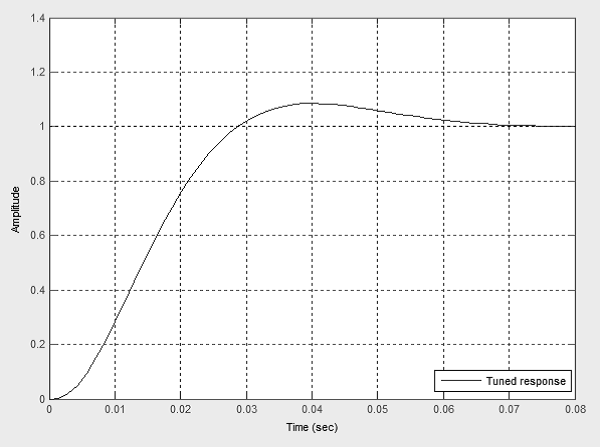
\includegraphics[width=.5\linewidth]{image11.png}

\textit{Tiroir en position travail}
\end{center}

On utilise les notations suivantes :
\begin{itemize}
\item $m_t$ : masse du tiroir ;
\item $S_t$ : section du tiroir à ses extrémités ;
\item $F_A$ et $F_B$ : efforts exercés par les deux ressorts de coefficient de raideur $k_t$ montés de part et d’autre
du tiroir du distributeur ;
\item $c_t$ : coefficient de frottement visqueux entre tiroir et cylindre.
\end{itemize}

Le principe fondamental de la dynamique appliqué au tiroir donne la relation suivante :
$$
m_t\dfrac{d^2z(t)}{dt^2} = -2k_tz(t) + 2S_t\Delta P(t) -c_t \dfrac{dz(t)}{dt}
$$

\fi


\subparagraph{}
\textit{Calculer la fonction de transfert $H_t(p)=\dfrac{Z(p)}{\Delta P(p)}$ 
où $Z(p)$ et $\Delta P(p)$ sont les transformées de Laplace de $z(t)$ et 
$\Delta P(t)$ en précisant l'hypothèse retenue.}
\ifprof
\begin{corrige}

En se plaçant dans les conditions de Heaviside, on peut transformer l'équation
dans le domaine de Laplace. On a donc : 
$$
m_t p^2 Z(p) = -2k_t Z(p) + 2 S_t \Delta P(p) - pc_t Z(p)
$$

Ainsi, 

$$
H_t(p)=\dfrac{Z(p)}{\Delta P(p)} = \dfrac{2S_t}{m_tp^2+c_tp+2k_t}
$$
\end{corrige}
\else
\fi

\subparagraph{}
\textit{Mettre cette fonction de transfert sous forme canonique et donner son ordre.}

\ifprof
\begin{corrige}

En factorisant par $2k_t$ on obtient : 
$$
H_t(p)= \dfrac{\dfrac{S_t}{k_t}}{1+\dfrac{c_t}{2k_t}p+\dfrac{m_t}{2k_t}p^2}
$$

\end{corrige}
\else
\fi
On admet pour finir que la pression d'utilisation $P_h(t)$ du fluide est proportionnelle au déplacement $z(t)$ du tiroir : $P_h(t) =K_4 z(t)$.

\subparagraph{}
\textit{\`A partir de toutes les informations précédentes (modélisation armature, buse/palette,
tiroir...), recopier et compléter le schéma-bloc de la servovalve donné ci-dessous, en précisant les
fonctions de transfert de chaque bloc (utiliser les notations algébriques).}

\ifprof
\begin{corrige}
On utilise les équation suivantes : 
$\theta(t)=K_1 i(t) \Leftrightarrow \Theta(p)=K_1 I(p)$, 
$\Delta S(t) = K_2 \theta (t) \Leftrightarrow  \Delta S(p) = K_2 \Theta (p)$,
$\Delta P(t) = K_3 \Delta S(t) \Leftrightarrow  \Delta P(p) = K_3 \Delta S(p)$,
$P_h(t)=K_4 z(t) \Leftrightarrow   P_h(p)=K_4 Z(p)$.

On en déduit ainsi le schéma bloc suivant :
\begin{center}
 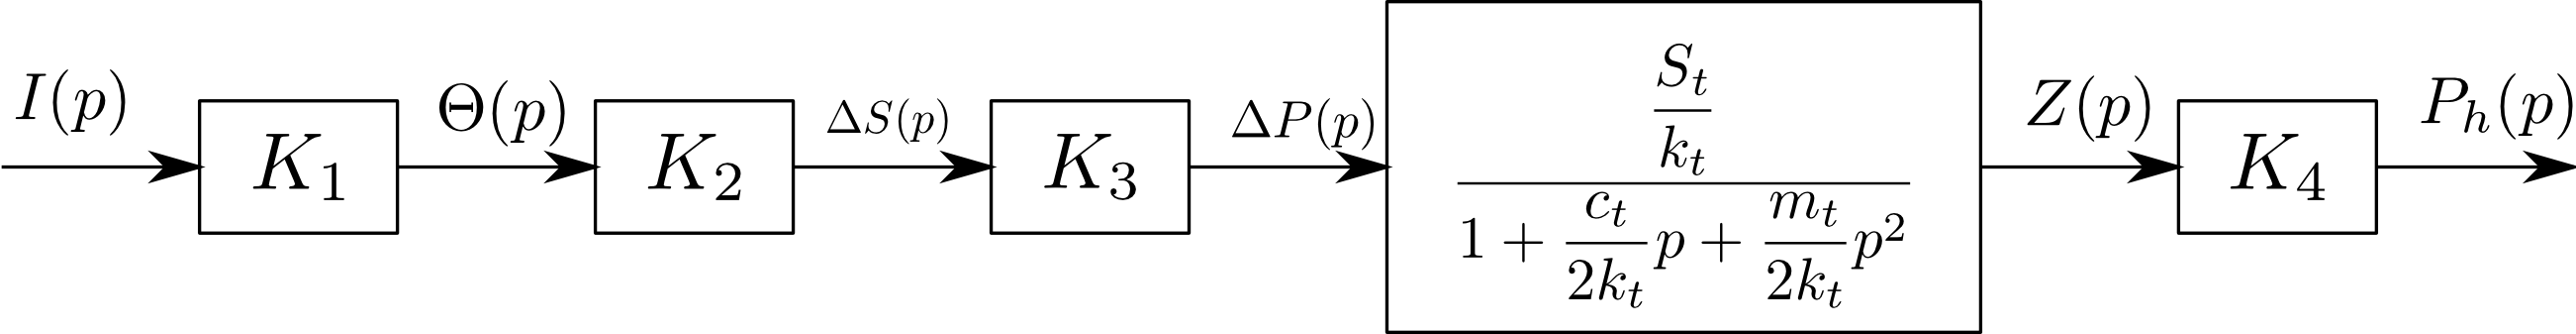
\includegraphics[width=.8\linewidth]{blocs2}
\end{center}
\end{corrige}
\else
\begin{center}
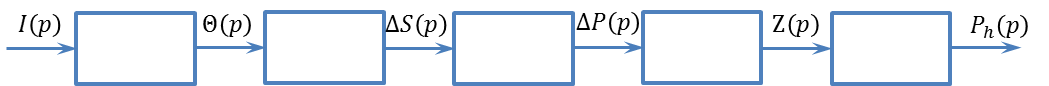
\includegraphics[width=.95\linewidth]{schema_bloc_vierge.png}
\end{center}
\fi



\subparagraph{}
\textit{En déduire la fonction de transfert $S_v(p)=\dfrac{P_h(p)}{I(p)}$ de la servovalve.}
\ifprof
\begin{corrige}
On en déduit directement : 
$$
S_v(p)=\dfrac{P_h(p)}{I(p)} = \dfrac{K_1 K_2 K_3 K_4
\dfrac{S_t}{k_t}}{1+\dfrac{c_t}{2k_t}+\dfrac{m_t}{2k_t}p^2}
$$
\end{corrige}
\else
\fi

\subparagraph{}
\textit{Montrer qu'elle peut se mettre sous la forme d'un système du second ordre :}
$$
S_v(p)=\dfrac{P_h(p)}{I(p)}=\dfrac{K_{sv}}{1+\dfrac{2\xi p}{\omega_0}+\dfrac{p^2}{\omega_0^2}}
$$
\textit{où on donnera les expressions littérales de $K_{sv}$, $\xi$ et $\omega_0$.}

\ifprof
\begin{corrige}
Par identification, on déduit de la question précédente : 

$
K_{SV} = K_1 K_2 K_3 K_4
\dfrac{S_t}{k_t}
$, $
\omega_0 = \sqrt{\dfrac{2k_t}{m_t}}
$,
$
\xi = \dfrac{c_t}{2\sqrt{2k_t m_t}}
$.

\end{corrige}
\else
\fi

On souhaite que la réponse à une entrée $i(t)$ de type échelon de valeur $i_0$ soit la plus rapide possible \textbf{sans toutefois produire de dépassement.}

\subparagraph{}
\textit{A quelle valeur de $\xi$ correspond cette spécification ?}
\ifprof
\begin{corrige}
Pour ne pas avoir de dépassement, il est nécessaire que $\xi \geq 1$. Le
système est le plus rapide lorsque $\xi=1$.
\end{corrige}
\else
\fi

\subparagraph{}
\textit{Démontrer que cette condition ne peut être satisfaite que si $k_t=\dfrac{c_t^2}{8m_t}$.}

\ifprof
$$
\xi = 1 \Leftrightarrow  c_t = 2\sqrt{2k_t m_t} \Leftrightarrow  k_t =
\dfrac{c_t^2}{8 m_t}
$$
\else
\fi

\subparagraph{}
\textit{Montrer alors que la fonction de transfert de la servovalve peut se mettre sous la forme :}
$$
S_v(p)=\dfrac{P_h (p)}{I(p)}=\dfrac{K_{sv}}{\left( 1+T_{sv} p\right)^2 }
$$
\textit{on donnera l'expression littérale de $T_{sv}$.}
\ifprof
\begin{corrige}

Lorsque $\xi=1$, le discriminant du dénominateur de la fonction
$S_v(p)$ est nul. En conséquence ce dénominateur possède une racine double. En
utilisant la formulation proposée, cette racine est égale à
$\dfrac{-1}{T_{sv}}$. En développant la fonction proposée, on peut donc
identifier $T_sv$ :
$
\left( 1+T_{sv} p\right)^2  = 1+\dfrac{2
p}{\omega_0}+\dfrac{p^2}{\omega_0^2}  \Leftrightarrow 1 + 2 T_{sv} p +T_{sv}^2
p^2 $
$= 1+\dfrac{2
p}{\omega_0}+\dfrac{p^2}{\omega_0^2}   
$

On a donc : 
$
T_{sv}=\dfrac{1}{\omega_0} $ 
$= \sqrt{\dfrac{m_t}{2k_t}} $
$ = \sqrt{\dfrac{m_t}{2\dfrac{c_t^2}{8 m_t}}} $
$= 2\dfrac{m_t}{c_t} $
\end{corrige}
\else
\fi


\subparagraph{}
\textit{Déterminer la réponse indicielle $P_h(t)$ pour une entrée échelon de valeur $i(t)=i_0 u(t)$.}

On rappelle que $\mathcal{L}\left(te^{-at}u(t)\right)=\dfrac{1}{\left(p+a\right)^2}$.

\ifprof
\begin{corrige}

On soumet le système à une entre échelon. En conséquence, on a : $
I(p)=\dfrac{i_0}{p}$.

On a alors $P_h(p)=\dfrac{i_0}{p}\dfrac{K_{sv}}{\left(1+T_{sv}p\right)^2}$.

En réalisant la décomposition en éléments simples, on a : $
P_h(p)=\dfrac{\alpha}{p}+\dfrac{\beta}{1+T_{sv}p}+\dfrac{\gamma}{\left(1+T_{sv}
p\right)^2}$.

En calculant $P_h(p)p$ et en posant $p=0$, on obtient $\alpha = K_{sv}i_0$.

En calculant $P_h(p)\left(1+T_{sv} p\right)^2$ et en posant
$p=-\dfrac{1}{T_{sv}}$, on obtient $\alpha = K_{sv}i_0$. On obtient alors
$\gamma = - K_{sv} T_{sv} i_0$.

Enfin, en calculant $\lim\limits_{p\to +\infty} p P_h(p)$ on obtient $\beta =
-K_{sv} T_{sv} i_0$.

Au final, on obtient : 
$
P_h(p) = K_{sv} i_0 \left( \dfrac{1}{p} - \dfrac{T_{sv}}{1+T_{sv}p} -
\dfrac{T_{sv}}{\left(1+T_{sv}p\right)^2} \right) 
$
$=
K_{sv} i_0
\left( 
\dfrac{1}{p}
-\dfrac{1}{\dfrac{1}{T_{sv}}+p}
-\dfrac{\dfrac{1}{T_{sv}}}{\left(\dfrac{1}{T_{sv}}+p\right)^2}
\right) 
$


En repassant dans le domaine temporel, on obtient :
$
P_h(t) = K_{sv} i_0 \left( 
1-e^{-\dfrac{-t}{T_{sv}}}
-\dfrac{t}{T_{sv}}e^{-\dfrac{-t}{T_{sv}}}
\right) u(t)
$
\end{corrige}
\else
\fi


\subsection*{Modélisation de l'accéléromètre}
\ifprof
\else
La centrale inertielle contient des accéléromètres qui permettent de mesurer les accélérations suivant les
trois directions $x_a$, $y_a$, $z_a$ d’un repère lié à l’avion.

L’accéléromètre renvoie au BSCU un signal électrique $u_a(t)$ image de l’accélération $a(t)$ suivant la
direction $x_a$. La tension $u_a(t)$ est convertie en grandeur numérique $a_m$ par un convertisseur analogique-numérique et rangée dans la mémoire du BSCU. 
\fi

\subsection*{Principe de l’accéléromètre}
\ifprof
\else

Un accéléromètre (voir figure ci-dessous) est constitué de deux solides
$S_1$ et $S_2$ :
\begin{itemize}
\item $S_1$, le corps, est lié à l’avion,
\item $S_2$ est lié à $S_1$ par l’intermédiaire d’un ressort de raideur $k_a$ et d’un frottement visqueux de valeur $c_a$.
\end{itemize}

\begin{center}
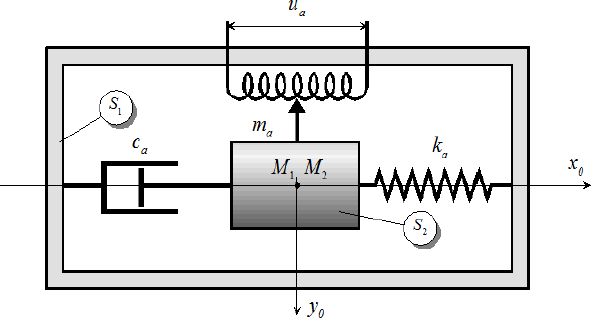
\includegraphics[width=.5\linewidth]{image12.png}

\textit{Accéléromètre en position repos}
\end{center}

On considère (voir figure ci-dessus) deux points $M_1$ et $M_2$ appartenant respectivement à $S_1$ et $S_2$. On note
$x_1(t)$ et $x_2(t)$ leurs coordonnées dans un repère 
$\left(O,\overrightarrow{x_0},\overrightarrow{y_0},\overrightarrow{z_0}\right)$.

On considère nulles les conditions initiales. En particulier, à l’état repos, $M_1$ et $M_2$ sont confondus.
Quand $S_1$ est animé d’un mouvement de translation suivant $x_0$, on note :
\begin{equation}
\varepsilon(t)=x_1(t)-x_2(t)
\end{equation}

\begin{equation}
a(t)=\dfrac{d^2x_1(t)}{dt^2} \text{ accélaration de } S_1
\end{equation}


\begin{center}
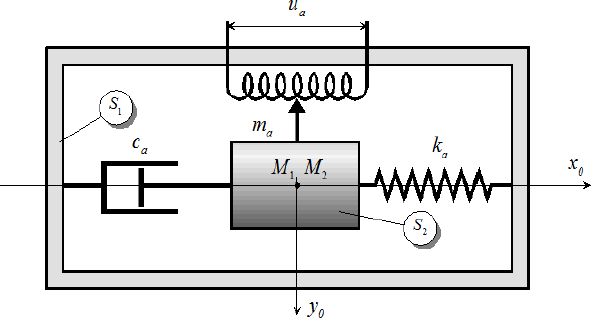
\includegraphics[width=.5\linewidth]{image12.png}

\textit{Accéléromètre en action}
\end{center}

D’autre part, par application du principe fondamental de la dynamique, on a :

\begin{equation}
m_a\dfrac{d^2x_2(t)}{dt^2}=c_a\left( \dfrac{dx_1(t)}{dt} - \dfrac{dx_2(t)}{dt}\right)
+k_a\left( x_1(t)-x_2(t)\right) 
\end{equation}

$\mathrm{avec} \quad m_a, c_a, k_a \quad \mathrm{constantes}$.

Le solide $S_2$ est relié à un potentiomètre qui renvoie une tension $u_a$ proportionnelle au déplacement $\varepsilon$ du solide $S_2$ par rapport à $S_1$. On note : 

\begin{equation}
u_a(t)=K_p \varepsilon(t)
\end{equation}

Finalement, le CAN (convertisseur analogique numérique) fournit la valeur $a_m$ telle que :
\begin{equation}
a_m(t) = K_{CAN} u_a (t) 
\end{equation}

\fi

\subparagraph{}
\textit{Déterminer les transformées de Laplace des expressions (1) à (5).}
\ifprof
\begin{corrige}

On obtient directement : 
$ \varepsilon(p)=X_1(p)-X_2(p)$, 
$ A(p)=p^2 X_1(p) $, 
$m_a p^2 X_2(p)=c_a \left( pX_1(p) - pX_2(p)\right)+k_a\left( X_1(p) -X_2(p) \right)$,
$U_a(p)=K_p \varepsilon(p)$, 
$A_m(p)=K_{CAN} U_a(p)$.
\end{corrige}



\else
\fi

\subparagraph{}
\textit{En déduire les transmittances $G_i$ du schéma bloc ci-après.}
\ifprof
\begin{corrige}
On a : 
$G_1(p) = \dfrac{X_1(p)}{A(p)}=\dfrac{1}{p^2}$.

D'après la troisième relation, on a :
$
X_2(p)\left( m_a p^2 +c_a p + k_a \right) = X_1(p) \left( c_a p + k_a  \right)
$
 et donc 
$
G_2(p) = \dfrac{X_2(p)}{X_1(p)} = \dfrac{c_a p + k_a}{m_a p^2 +c_a p + k_a}
$,
$
G_3(p) = \dfrac{U_a(p)}{\varepsilon(p)} = K_p
$
et
$
G_4(p) = \dfrac{A_m(p)}{U_a(p)} = K_{CAN}
$.

\end{corrige}
\else
\fi

\begin{center}
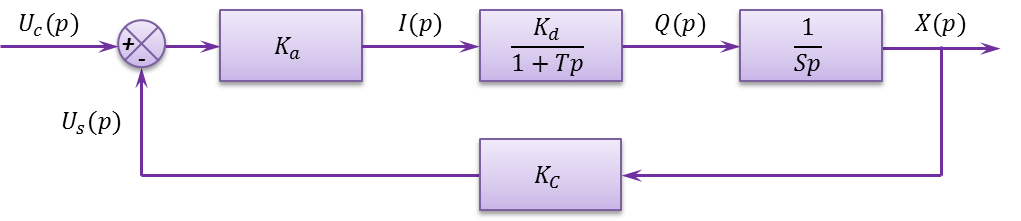
\includegraphics[width=.8\linewidth]{schema_bloc.png}
\end{center}

\subparagraph{}
\textit{En déduire la fonction de transfert $\dfrac{A_m(p)}{A(p)}$ et montrer quelle peut se mettre sous la
forme :}
$$
\dfrac{A_m(p)}{A(p)} = \dfrac{K_{acc}}{1+2\dfrac{\xi_a p}{\omega_a} + \dfrac{p^2}{\omega_a^2}}
$$
\textit{Donner les expressions de $K_{acc}$, $\xi_a$ et $\omega_a$.}

\ifprof
\begin{corrige}

D'après le schéma bloc, on a : 
$$
 \dfrac{A_m(p)}{A(p)} = G_1 \left(1 - G_2 \right) G_3 G_4 
$$

D'où 
$
 \dfrac{A_m(p)}{A(p)} = \dfrac{1}{p^2} \left( 1- \dfrac{c_a p + k_a}{m_a p^2
+c_a p + k_a} \right)  K_p K_{CAN} $
$=\dfrac{K_p K_{CAN} m_a}{m_a p^2 +c_a p + k_a}
$

En mettant la fonction cette fonction de transfert sous la forme canonique :
$
\dfrac{A_m(p)}{A(p)} = \dfrac{\dfrac{K_p K_{CAN} m_a}{k_a}}{\dfrac{m_a}{k_a}p^2
+ \dfrac{c_a}{k_a}p+1}
$.

Au final : $K_{acc} = \dfrac{K_p K_{CAN} m_a}{k_a}$, 
$ \xi_a = \dfrac{c_a}{2\sqrt{k_a m_a}}$
et $
\omega_a = \sqrt{\dfrac{k_a}{m_a}}
$.
\end{corrige}
\else
\fi

\subparagraph{}
La figure ci-dessous donne la réponse indicielle (entrée unitaire) de l'accéléromètre.
Identifier les valeurs des constantes $K_{acc}$ , $\xi_a$ et $\omega_a$ (On pourra utiliser les abaques donnés en annexe).
\ifprof
\begin{corrige}
D'après le tracé de la réponse indicielle avec une entrée unitaire, on observe
bien la réponse d'un système du second ordre (tangente horizontale et un
dépassement).

L'entrée est unitaire et le système tend vers 1 lorsque t tend vers l'infini.
En conséquence on a $K_{acc}=1$.

La valeur du premier dépassement est de 1,05. En conséquence le dépassement est
de 5\%. D'après l'abaque du dépassement relatif, on a donc : $\xi_a=0,7$. 

En utilisant l'abaque donnant $t_r \omega_0$ en fonction de $\xi$ on lit que 
$t_r \omega_0 = 3$. 


Enfin, en mesurant le temps de réponse à 5\% on a $t_r \simeq 0,03 s.$. En
conséquence : $\omega_a = \dfrac{3}{0,03}\simeq 100 \; rad/s$.

Réponse acceptée : pour le temps de réponse à 5\% $t_r = 0,045 s.$. En
conséquence : $\omega_a = \dfrac{3}{0,045}\simeq 66\;  rad/s$.

\end{corrige}
\else
\fi



\ifprof
\else
\begin{center}
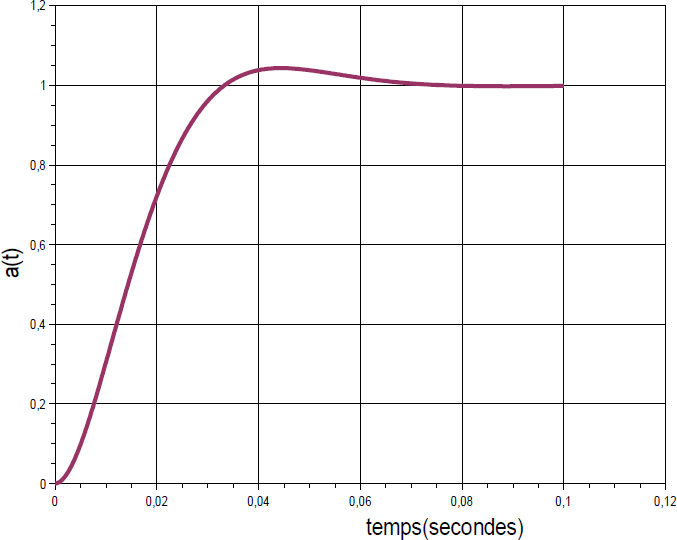
\includegraphics[width=.8\linewidth]{image15.png}
\end{center}
\fi

\section*{Étude de l'asservissement global}
\ifprof
\else
La boucle d'asservissement en décélération est donnée ci-après :

\begin{center}
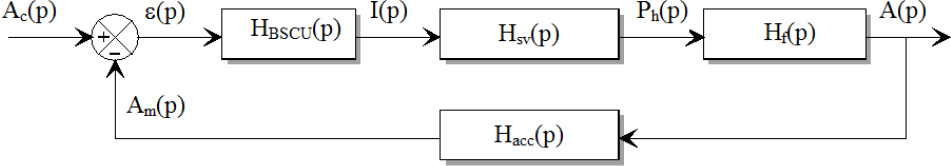
\includegraphics[width=.8\linewidth]{image16.png}
\end{center}

avec : 
$H_{sv} (p)=\dfrac{K_{sv}}{\left(1+T_{sv} p\right)^2}$, 
$H_{acc}(p)=\dfrac{K_{acc}}{1+\dfrac{2\xi_a }{\omega_a}p+\dfrac{p^2}{\omega_a^2}}$, 
$H_f(p)=K_f$, 
$H_{BSCU}(p)=K_c$.
\fi

\subparagraph{}
\textit{Exprimer sous forme canonique la fonction de transfert en boucle ouverte. En déduire
l’ordre, la classe et le gain de la $\text{\text{FTBO}}(p)$.}
\ifprof
\begin{corrige}
Par définition, la \text{FTBO} s'exprime par la relation :
$
\text{\text{FTBO}}(p)=H_{BSCU} \cdot H_{SC}(p) \cdot H_f(p) \cdot H_{acc}(p) $ $=
\dfrac{K_cK_{SV}K_fK_{acc}}{\left( 1+T_{sv}p
\right)^2\left(1+\dfrac{2\xi_a}{\omega_a}p+\dfrac{p^2}{\omega_a^2}\right)}
$

Le gain de la \text{FTBO} est donné par le numérateur : $K_cK_{SV}K_fK_{acc}$. 

L'ordre de la \text{FTBO} est donné par le monôme de plus haut degré : l'ordre est
donc de 4 (lorsqu'on développe le système).

La classe du système est donné par le nombre d'intégrateur présent au
dénominateur. Ici, $p$ ne peut pas être mis en facteur du dénominateur. La
classe est donc de 0.


\end{corrige}
\else
\fi

\subparagraph{}
\textit{Exprimer l'écart $\varepsilon(p)$ en fonction de $a_c(p)$ et de la $\text{FTBO}(p)$.}
\ifprof
\begin{corrige}
D'après le schéma bloc, on a : 
$\varepsilon(p) = A_c(p)-A_m(p) =A_c(p)-\varepsilon(p)\cdot \text{FTBO}(p)$
 $\Leftrightarrow
\varepsilon(p) \left( 1-\text{FTBO}(p)\right) = A_c(p)
$

On a donc :
$$
\varepsilon(p)  = \dfrac{A_c(p)}{\left( 1-\text{FTBO}(p)\right)}
$$

\end{corrige}
\else
\fi

\subparagraph{}
\textit{En déduire l'écart en régime permanent à une entrée de type échelon d'accélération
$a_c (t)=a_cu (t)$. Que peut on dire de la performance de précision pour ce correcteur ?}
\ifprof
\begin{corrige}
L'écart est donné par la fonction $\varepsilon$. L'écart en régime permanent
est donné par la limite de $\varepsilon(t)$ en l'infini. D'après le théorème de
la valeur finale on a donc :

$$
\lim\limits_{t\to +\infty} \varepsilon(t) = \lim\limits_{p\to 0}
p\varepsilon(p) =  \lim\limits_{p\to 0} \dfrac{p A_c(p)}{\left(
1-\text{FTBO}(p)\right)}
$$


L'entrée est un échelon d'accélération d'amplitude $a_c$. En conséquence : $A_c (p)=\dfrac{a_c}{p}$ et
$
\lim\limits_{t\to +\infty} \varepsilon(t) = \lim\limits_{p\to 0}
\dfrac{a_c}{p} \dfrac{p}{1+\text{FTBO}(p)}
$.

Or, $
 \lim\limits_{p\to 0} \text{FTBO}(p) = K_cK_{SV}K_fK_{acc}
$.

En conséquence, 
$
\lim\limits_{t\to +\infty} \varepsilon(t) = \dfrac{a_c}{1+K_cK_{SV}K_fK_{acc}}
$.

L'écart statique de ce système n'étant pas nul, le système n'est donc pas
précis.

\end{corrige}
\else
\fi


\subparagraph{}
\textit{On utilise un correcteur (correcteur PI) plus évolué de fonction de transfert
$H_{BSCU}(p)=K_i\dfrac{1+T_i p}{p}$, déterminer à nouveau l'écart en régime permanent et conclure sur ce choix de correcteur.}
\ifprof
\begin{corrige}

Il suffit dans un premier temps de calculer la limite quand $p$ vers 0 
de la nouvelle \text{FTBO}. 

Cette \text{FTBO} vaut :

$$
\text{FTBO}(p)=
\dfrac{K_cK_{SV}K_fK_{acc}}{\left( 1+T_{sv}p
\right)^2\left(1+\dfrac{2\xi_a}{\omega_a}p+\dfrac{p^2}{\omega_a^2}\right)}
\dfrac{K_i\left(1+T_i p\right)}{p}
$$

On a alors :
$$
\lim\limits_{p\to+\infty}\text{FTBO}(p)=+\infty
$$
En conséquence, 
$$
\lim\limits_{t\to +\infty} \varepsilon(t) = \dfrac{1}{1+\infty} = 0
$$

L'écart statique étant nul, le système est donc précis.

\end{corrige}
\else
\fi

\ifprof
\else
\begin{center}
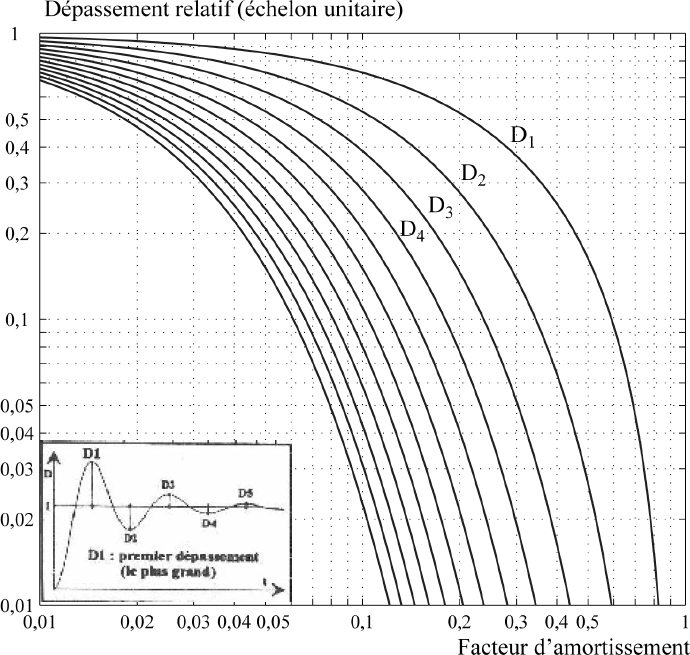
\includegraphics[width=.75\linewidth]{image17.png}
\end{center}

\begin{center}
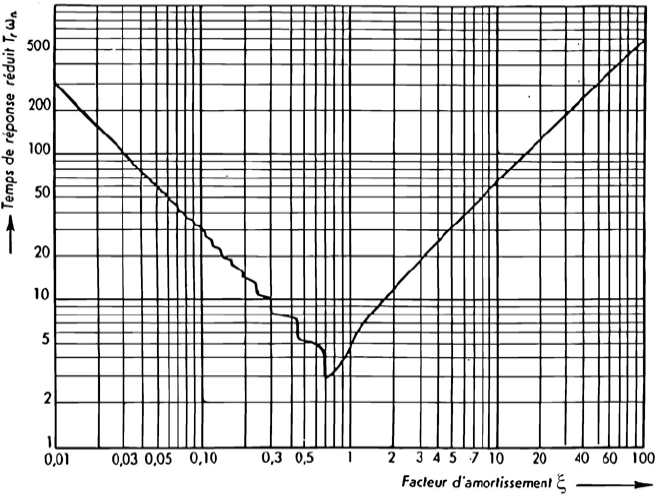
\includegraphics[width=.75\linewidth]{image18.png}
\end{center}
\fi
%\begin{center}
%\Large\textsc{-- Bon WeekEnd --}
%\end{center}


%\newpage{}

%\section*{Documents réponse}
%\begin{center}
%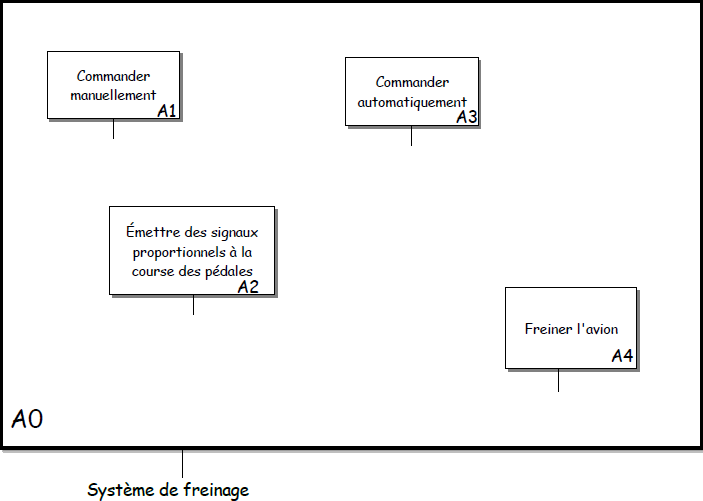
\includegraphics[width=\linewidth]{image19.png}
%\end{center}

%\begin{center}
%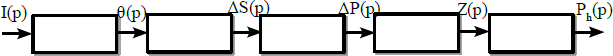
\includegraphics[width=\linewidth]{image20.png}
%\end{center}


\ifprof
\else
\end{multicols}
\fi
